\documentclass[a4paper, 12pt]{article}
\usepackage[utf8]{inputenc}
\usepackage[top=2cm, bottom=2cm, left=2cm, right=2cm]{geometry}
\usepackage{graphicx}
\graphicspath{{../src/data/graphs/}}
\usepackage{caption}
\usepackage{subcaption}
\usepackage{float}
\DeclareGraphicsExtensions{.jpg,.png}
\renewcommand{\figurename}{Fig.}

\usepackage{amsmath, amsfonts, amssymb, xcolor}
\usepackage{forest}

\begin{document}

\begin{titlepage}
	\begin{center}
		\line(1,0){400} \\
		[0.25in]
		\huge{\bfseries Exercício Programa I - Relatório} \\
		[0.01in]
		\line(1,0){300} \\
		[0.5cm]
		\textsc{\Large \bfseries MAC0219 - Programação Concorrente e Paralela} \\
		[1.5cm]
		\textsc{\large Prof.: Alfredo Goldman}\\
		\textsc{\large Monitor: Diogo Pina}\\
		[12cm]
	\end{center}
	\begin{flushright}
		\textsc{David de Barros Tadokoro}\\
		\textsc{NºUSP: 10300507}\\
		\textsc{Fernando Henrique Junqueira}\\
		\textsc{NºUSP: 11795888}\\
		\textsc{Julho de 2022}
	\end{flushright}
\end{titlepage}

\newpage

\section{Sobre a Entrega}

O diretório onde se encontra o arquivo \texttt{mac0219\_ep1\_10300507-11795888.pdf} (este relatório) deve ter a seguinte hierarquia de arquivos:\\

\begin{forest}
for tree={
    font=\ttfamily,
    grow'=0,
    child anchor=west,
    parent anchor=south,
    anchor=west,
    calign=first,
    edge path={
      \noexpand\path [draw, \forestoption{edge}]
      (!u.south west) +(7.5pt,0) |- node[fill,inner sep=1.25pt] {} (.child anchor)\forestoption{edge label};
    },
    before typesetting nodes={
      if n=1
        {insert before={[,phantom]}}
        {}
    },
    fit=band,
    before computing xy={l=15pt},
  }
[mac0219\_ep1\_10300507-11795888/
  [src/
    [mandelbrot\_seq.c]
    [mandelbrot\_seq\_mod.c]
    [mandelbrot\_omp.c]
    [mandelbrot\_pth.c]
  ]
  [data/
    [graphs/]
    [mandelbrot\_seq/]
    [mandelbrot\_seq\_mod/]
    [mandelbrot\_omp/]
    [mandelbrot\_pth/]
  ]
  [mac0219\_ep1\_10300507-11795888.pdf]
]
\end{forest}\\

O diretório \texttt{src/} contém os códigos fontes das implementações pedidas pelo enunciado. Além das duas implementações paralelizadas em OpenMP e em Pthreads, também incluímos o arquivo \texttt{mandelbrot\_seq\_mod.c}, que se refere a implementação sequencial que não usa operações de E/S nem de alocação de memória. Na prática, este código é uma cópia exata do código sequencial original, apenas com comentários em três linhas que resultavam nessas operações.\\

O diretório \texttt{data/} contém todos os dados usados na geração e análise dos resultados. Os diretórios inciados com \texttt{data/mandelbrot\_} contém os arquivos \texttt{.csv} referentes aos gráficos gerados.  O diretório \texttt{data/graphs/} contém todos estes gráficos (que serão expostos neste relatório).\\

\section{Metodologia}

Após termos confirmado que as implementações paralelizadas estavam corretas, passamos a realização dos experimentos e a coleta de dados.\\

Antes de descrever a metodologia, iremos expor o ambiente computacional (i.e. a máquina) onde estes experimentos foram realizados:
\begin{itemize}
\item CPU: AMD Ryzen 5 1500X Quad-Core:
\begin{itemize}
\item Cores: 4 físicos (8 núcleos lógicos)
\item Frequência do Clock: 3.6GHz
\item Índice BogoMIPS: 6985.90
\item Caches: L1 64K; L2 512K; L3 8192K
\end{itemize}
\item Memória Principal: 8GB RAM DDR4
\item Sistema Operacional: Ubuntu 18.04 LTS
\end{itemize}
\hfill

Para gerar os arquivos \texttt{.csv}, adaptamos o script em bash \texttt{run\_measurements.sh} fornecido junto ao enunciado. Apenas adicionamos o caso sequencial modificado e manipulamos as informações devolvidas pelo comando \texttt{perf} usando os programas \texttt{sed} e \texttt{grep}, para filtrarmos as informações de interesse num formato desejado (\texttt{.csv}).\\

\noindent\begin{small}
(\textbf{Obs.:} Na seção \ref{section:estrutura}, a estrutura destes dados, bem como a dos gráficos, é exposta em detalhes.)
\end{small}\\

Em nossos testes, cada comando \texttt{perf} realizou 10 execuções por dado, isto é, para cada ponto considerado em nossos gráficos (ou linha no \texttt{.csv}), tivemos um intervalo de confiança correspondente gerado pelo \texttt{perf}.\\

Nos casos sequenciais (original e modificado), para cada região do conjunto de Mandelbrot (\textit{Full}, \textit{Seahorse}, \textit{Elephant} e \textit{Triple Spiral}), extraímos 10 dados, cada um referente a um dos 10 tamanhos de entrada (de 16 até 8192).\\

Já nos casos paralelos, para cada uma das regiões e cada um dos números de threads (1, 2, 4, ... e 32 threads), extraímos 10 dados, cada um referente a um dos 10 tamanhos de entrada (de 16 até 8192).\\

Coletados os dados no formato \texttt{.csv}, utilizamos um script na linguagem Octave para gerarmos os gráficos para análise. Este script une os casos sequenciais em um gráfico só, para cada região.\\

\section{Estrutura dos dados e dos gráficos}\label{section:estrutura}

Como dito, os dados foram armazenados em 16 arquivos \texttt{.csv}, 4 para cada caso (sequencial original, sequencial modificado, paralelizado com OpenMP e paralelizado com Pthreads), sendo cada um destes 4 referentes a uma região contemplada do conjunto de Mandelbrot.\\

Estes arquivos \texttt{.csv} têm suas colunas estruturadas da seguinte forma:
\begin{itemize}
\item Coluna 1: Número de threads
\item Coluna 2: Tamanho da entrada
\item Coluna 3: Tempo médio de execução em segundos (\texttt{perf})
\item Coluna 4: Desvio padrão do tempo de execução em segundos (\texttt{perf})
\item Coluna 5: Desvio padrão do tempo de execução em porcentagem (\texttt{perf})
\end{itemize}

É importante frisar como cada linha destes arquivos descreve um intervalo de confiança (informação que não foi embutida nos gráficos pela legibilidade).\\

Os casos sequenciais, por não variarem o número de threads, possuem apenas 10 dados por região, ou seja, apenas 10 linhas por arquivo. Já os casos paralelizados, possuem 60 dados por região (devido as 6 variantes de números de threads), ou seja, 60 linhas por arquivo.\\

Sobre os gráficos, temos 4 gráficos referentes aos casos sequenciais e 8 gráficos referentes aos casos paralelizados. Cada gráfico contempla uma região do conjunto de Mandelbrot.\\

Nos gráficos sequenciais, temos 2 linhas, uma referente ao sequencial com operações de E/S e alocação de memória e outra referente ao sequencial sem estas operações (modificado). Já nos gráficos paralelizados, temos 6 linhas, cada uma referente a um número de threads.\\

\section{Resultados}

Nesta seção, iremos expor os resultados, isto é, os gráficos que nos possibilitarão inferir sobre os efeitos de paralelizarmos ou não um código.\\

\subsection{Casos Sequenciais}

\begin{figure}[H]
	\centering
	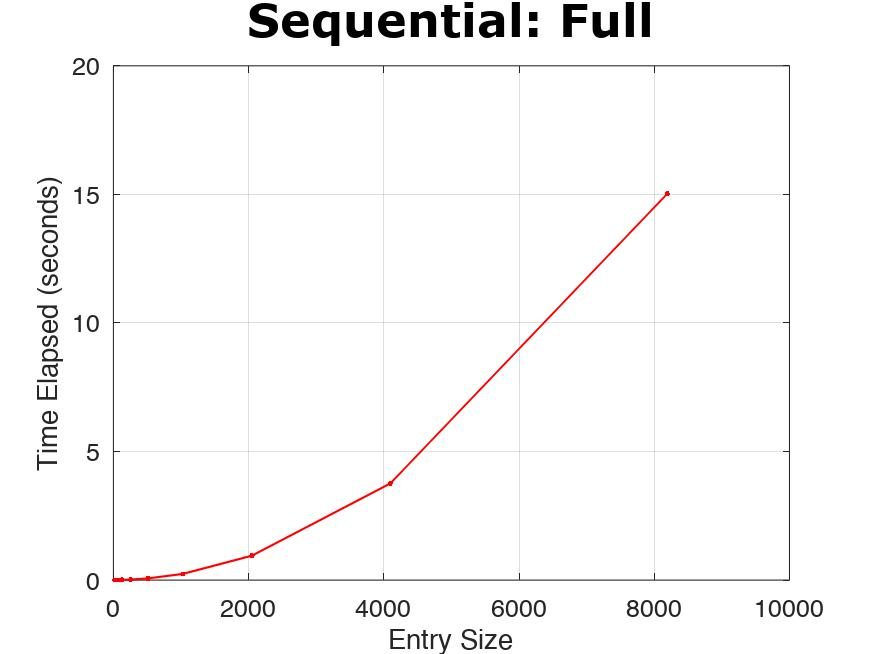
\includegraphics[scale=0.45]{seq_full}
	\caption{Caso sequencial na região \textit{Full}.}
\end{figure}

\begin{figure}[H]
	\centering
	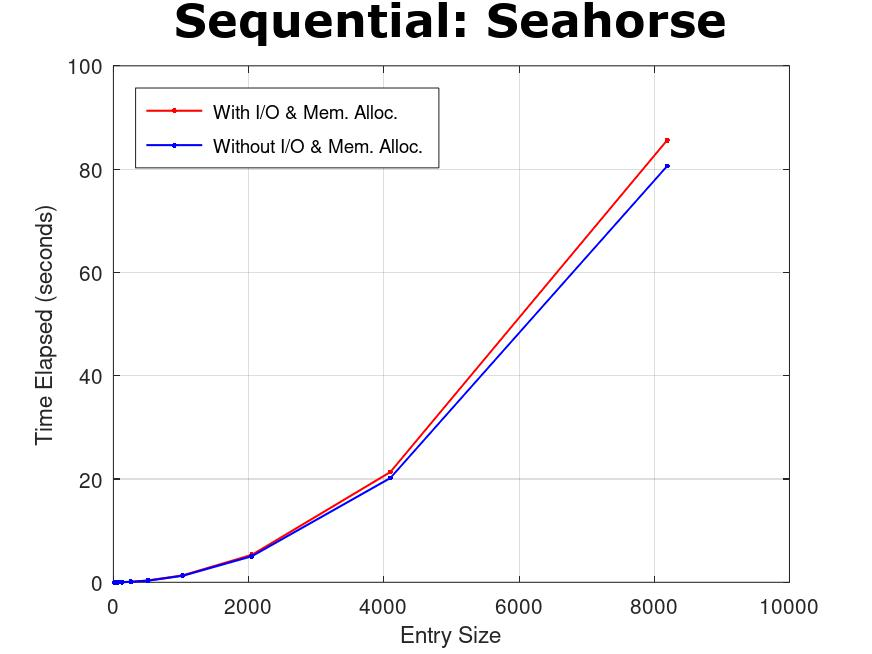
\includegraphics[scale=0.45]{seq_seahorse}
	\caption{Caso sequencial na região \textit{Seahorse}.}
\end{figure}

\begin{figure}[H]
	\centering
	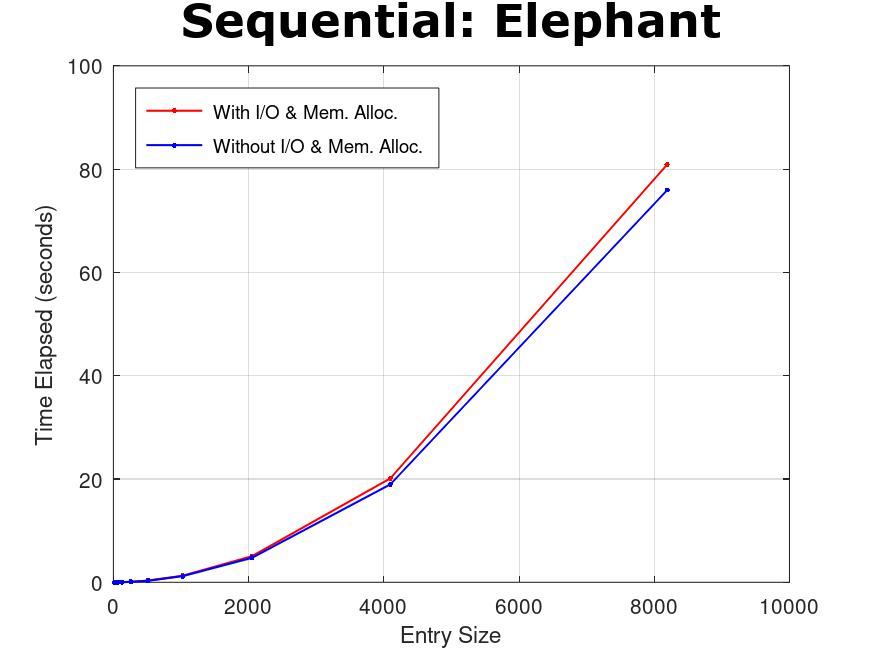
\includegraphics[scale=0.45]{seq_elephant}
	\caption{Caso sequencial na região \textit{Elephant}.}
\end{figure}

\begin{figure}[H]
	\centering
	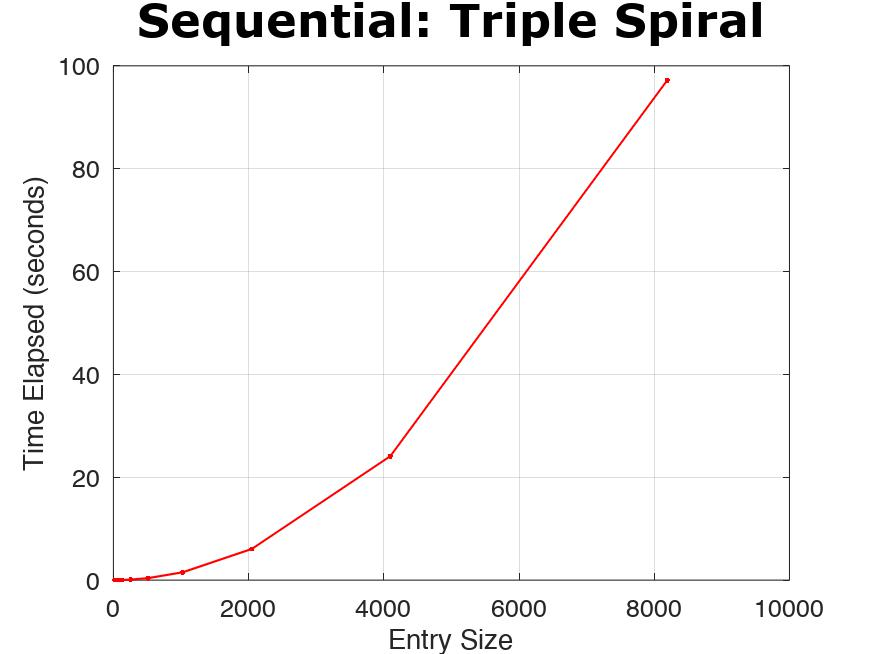
\includegraphics[scale=0.45]{seq_triple_spiral}
	\caption{Caso sequencial na região \textit{Triple Spiral}.}
\end{figure}

\subsection{Caso OpenMP}

\begin{figure}[H]
	\centering
	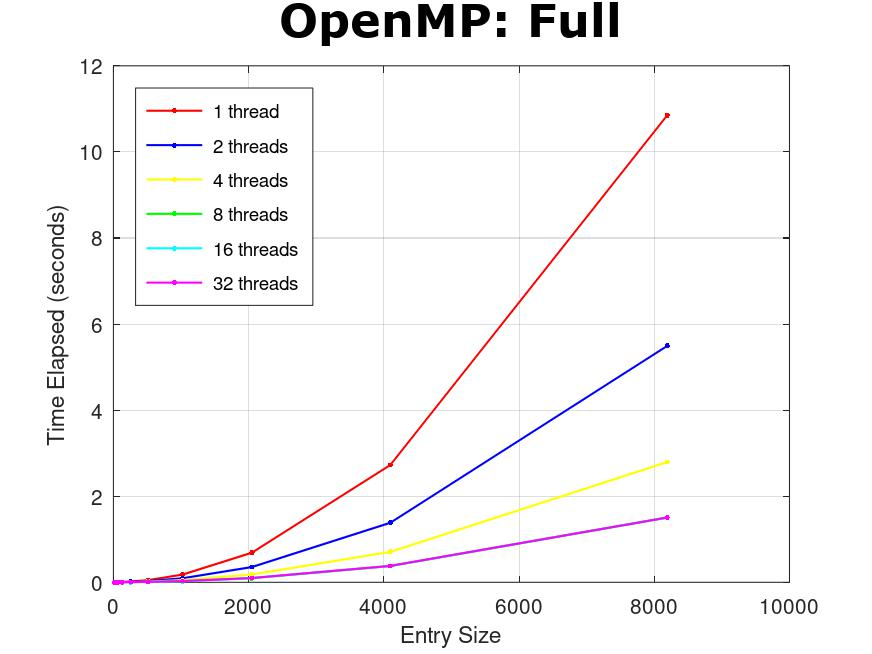
\includegraphics[scale=0.45]{omp_full}
	\caption{Caso OpenMP na região \textit{Full}.}
\end{figure}

\begin{figure}[H]
	\centering
	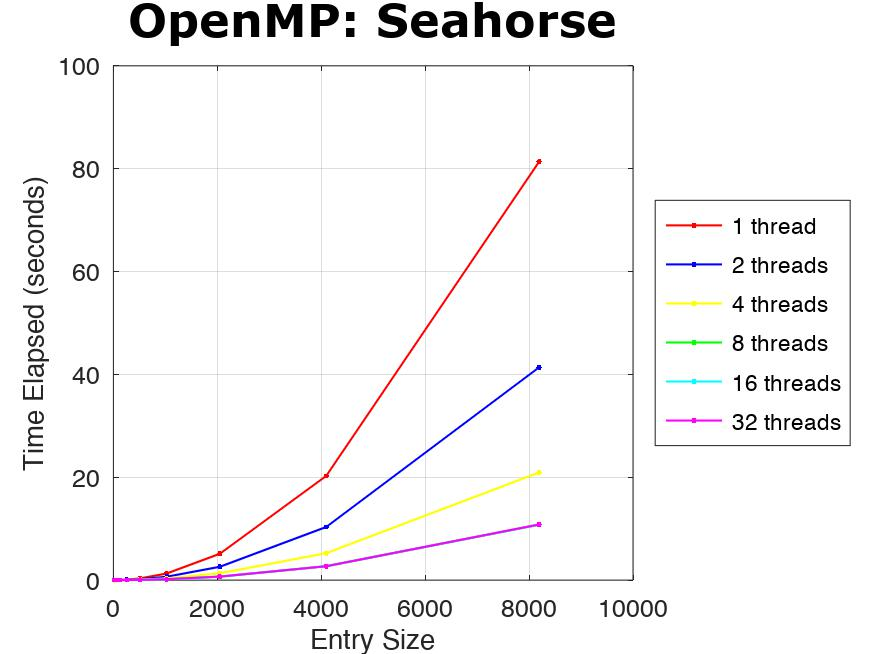
\includegraphics[scale=0.45]{omp_seahorse}
	\caption{Caso OpenMP na região \textit{Seahorse}.}
\end{figure}

\begin{figure}[H]
	\centering
	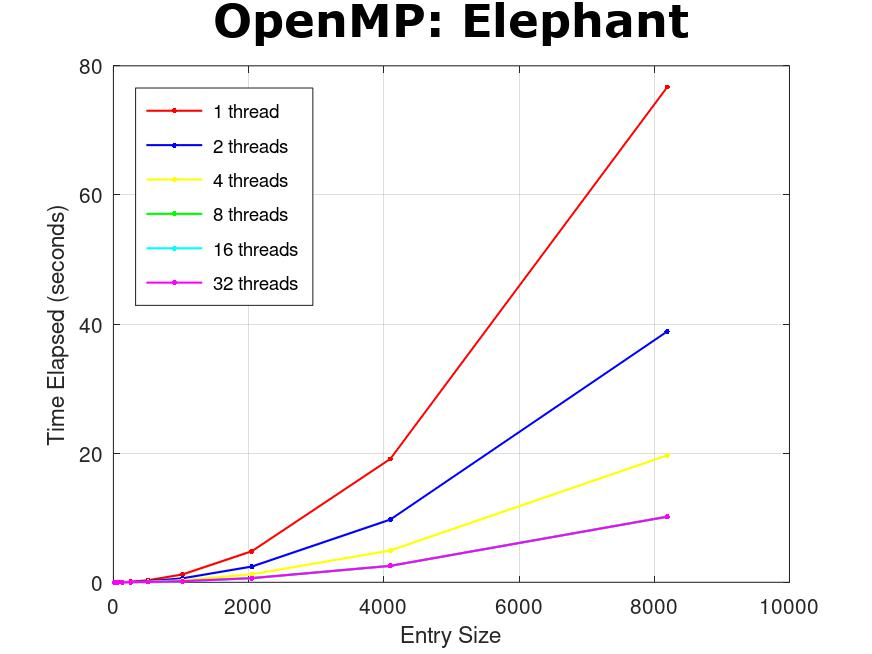
\includegraphics[scale=0.45]{omp_elephant}
	\caption{Caso OpenMP na região \textit{Elephant}.}
\end{figure}

\begin{figure}[H]
	\centering
	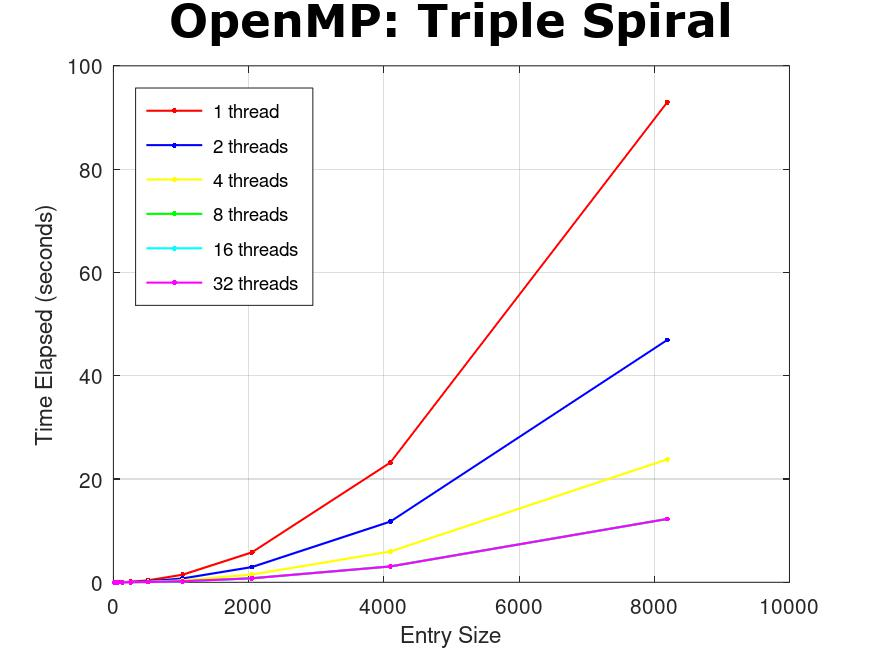
\includegraphics[scale=0.45]{omp_triple_spiral}
	\caption{Caso OpenMP na região \textit{Triple Spiral}.}
\end{figure}

\subsection{Caso Pthread}

\begin{figure}[H]
	\centering
	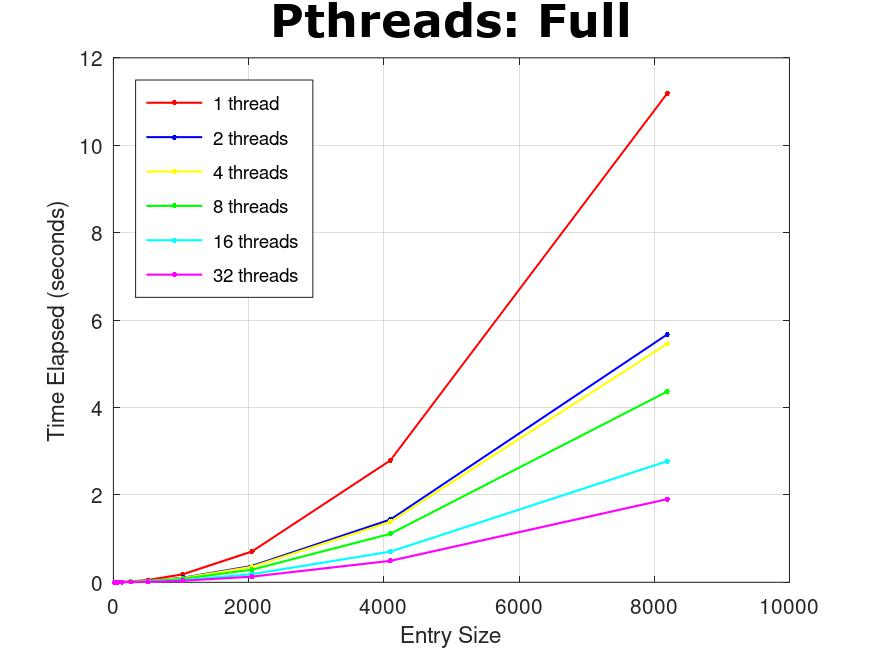
\includegraphics[scale=0.45]{pth_full}
	\caption{Caso Pthread na região \textit{Full}.}
\end{figure}

\begin{figure}[H]
	\centering
	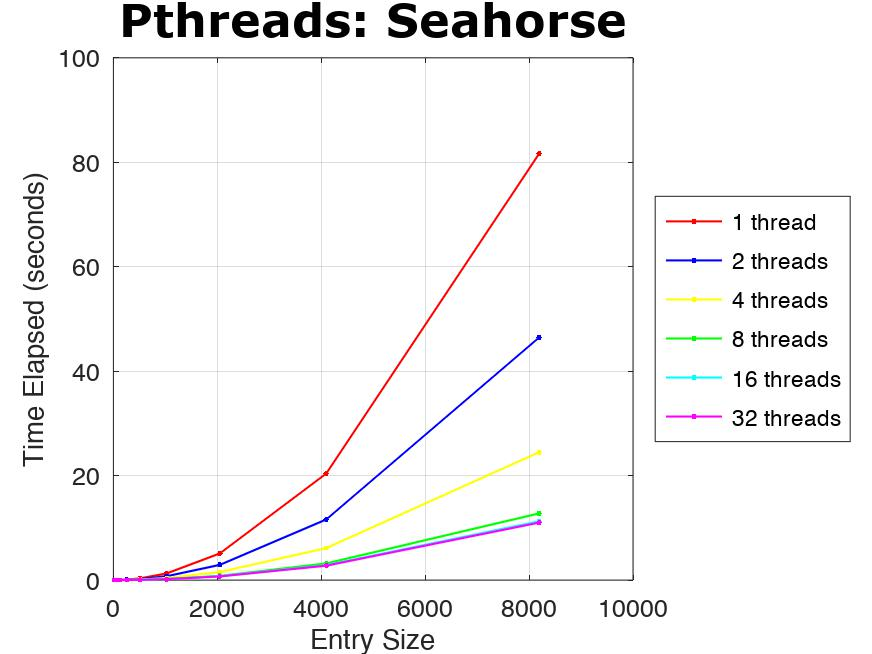
\includegraphics[scale=0.45]{pth_seahorse}
	\caption{Caso Pthread na região \textit{Seahorse}.}
\end{figure}

\begin{figure}[H]
	\centering
	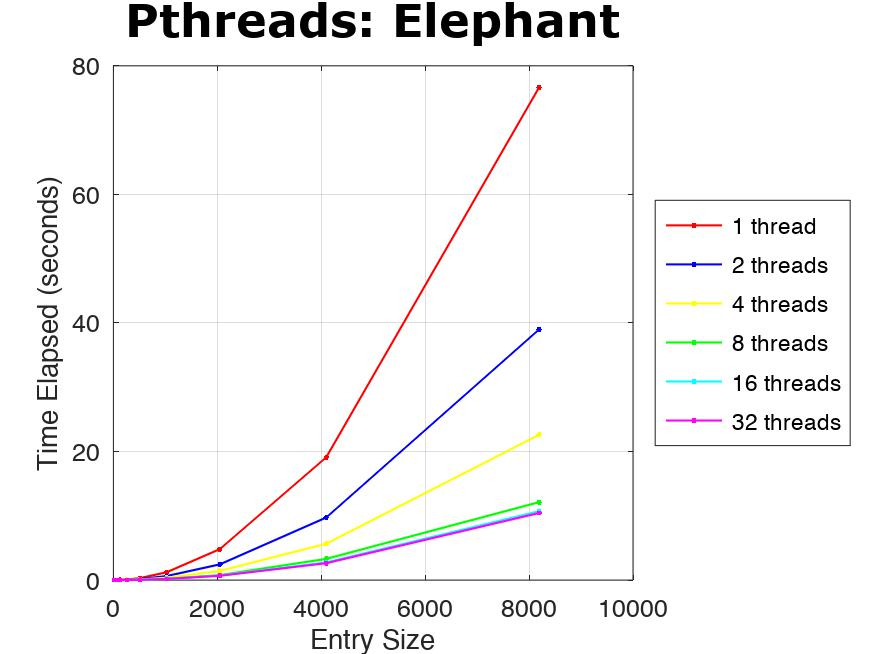
\includegraphics[scale=0.45]{pth_elephant}
	\caption{Caso Pthread na região \textit{Elephant}.}
\end{figure}

\begin{figure}[H]
	\centering
	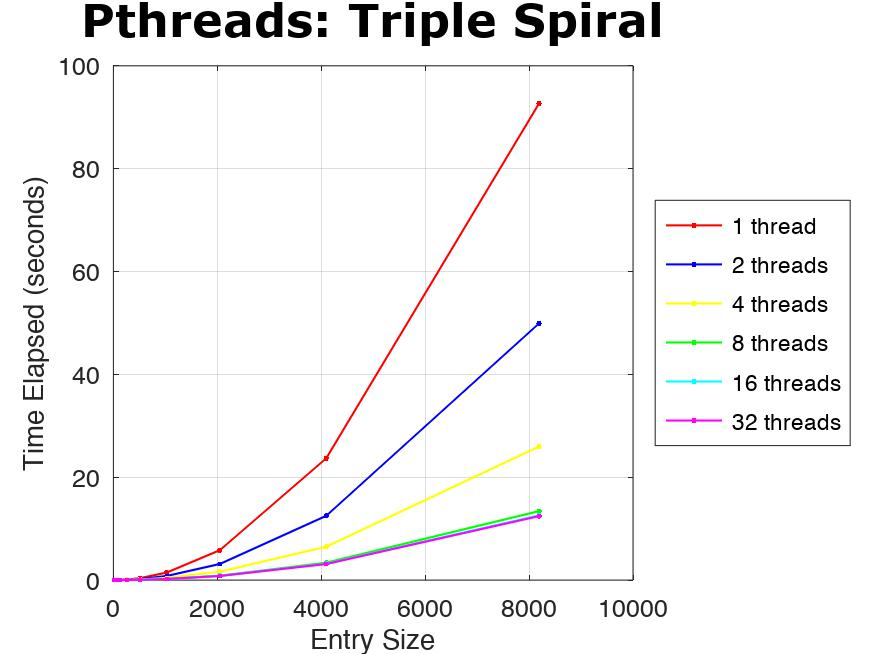
\includegraphics[scale=0.45]{pth_triple_spiral}
	\caption{Caso Pthread na região \textit{Triple Spiral}.}
\end{figure}
\hfill\\

\section{Análise}

Nesta seção, iremos tecer comentários comparativos entre os casos e tentar inferir o motivo das tendências que os resultados mostraram. Além disso, iremos discutir as particularidades de cada um dos casos.\\

\subsection{Comparações Gerais}

Primeiramente, note como os casos OpenMP, Pthread e sequencial modificado tem, virtualmente, o mesmo comportamento no caso de 1 thread só. Isto faz sentido, pois o caso sequencial modificado é, conceitualmente, a mesma situação dos casos paralelizados com uma única thread.\\

Em segundo lugar, veja como, de fato, os casos paralelizados tendem a ter um tempo de execução inversamente proporcional ao número de threads. Claro que há um limite inferior, mas é claro como a paralelização feita resultou em um ganho de performance grande. Por exemplo, somente de 1 para 2 threads, tanto no caso OpenMP, quanto no caso Pthreads, temos uma queda de quase 50\% no tempo de execução, de forma consistente para todas as regiões.\\

De forma comparativa, o caso OpenMP teve uma performance melhor que o caso Pthread, apesar de a diferença ter sido não muito expressiva. Poderíamos até dizer que, estatisticamente, ambas as implementações do programa tem a mesma performance. No entanto, o caso OpenMP aparente ter uma vantagem em relação ao caso Pthread, e isso será discutido na subseção dedicada ao OpenMP.\\

Para todos os casos, o tempo de execução é exponencialmente proporcional ao tamanho da entrada. Isto é esperado, pois uma entrada $e$ resulta em $e^2$ pixels (ou pontos) manipulados, e, portanto, uma entrada $e+1$ resulta em $(e+1)^2$ pixels (ou pontos) manipulados. Como o tempo de execução pode ser considerado proporcional ao número de pixels manipulados, vemos como, de fato, a tendência e quadrática em relação ao tamanho da entrada.\\

Também global a todos os casos, é a influência da região do conjunto de Mandelbrot no tempo de execução. Em consistência com os resultados, podemos classificar a "complexidade" das regiões de forma decrescente:
\begin{itemize}
\item 1. \textit{Triple Spiral}
\item 2. \textit{Seahorse}
\item 3. \textit{Elephant}
\item 4. \textit{Full}
\end{itemize}

Vale notar como a região \textit{Full} tem um tempo de execução, substancialmente, menor que o das outras regiões. A região \textit{Full}, também é a que possui um gradiente "menos contínuo", no sentido de que a borda do conjunto é mais bem definida, e, portanto, o número médio de iterações por ponto é menor (pois a maioria deles cumpre uma condição de escape antes do máximo de iterações). Baseado nisso, podemos dizer que a ordem da lista acima também corresponde ao "nível de detalhe do gradiente" ou ao "nível de complexidade média dos pontos".

\subsection{Analisando o caso sequencial}

Em particular, a única informação que o caso sequencial no permite inferir é como as operações de E/S e alocação de memória tem um custo fixo. Repare, nas figuras 1 a 4, como a diferença para uma entrada de 8192 é de aproximadamente 3 segundos para qualquer uma das regiões do conjunto.\\

Logicamente, com tamanhos diferentes de entrada a diferença não é por volta dos 3 segundos, mas ela é consistente para todas as regiões. Mas, se a complexidade varia de acordo com a região, esta diferença não deveria ser influenciada pela região também? A resposta para esta pergunta deveria ser sim, mas só se este custo não fosse fixo. Portanto, com base nisto, podemos inferir que ele é fixo e tende a ser menos relevante em tempos de execução grandes.

\subsection{Analisando o caso OpenMP}

Um fato é notável nos resultados do caso OpenMP: as linhas correspondentes a 8 e 16 threads (linhas verde e ciano) não são visíveis nos gráficos. Podemos dizer que não são visíveis, pois elas estão, de fato, no gráfico. No entanto, elas se sobrepõe a linha que corresponde a 32 threads (linha rosa) e, como esta linha é a última a ser plotada, esta é a única que é visível. Usando a ferramenta de zoom arbitrário do Octave, podemos confirmar que estas linhas se encontram, de fato, no gráfico:

\begin{figure}[H]
	\centering
	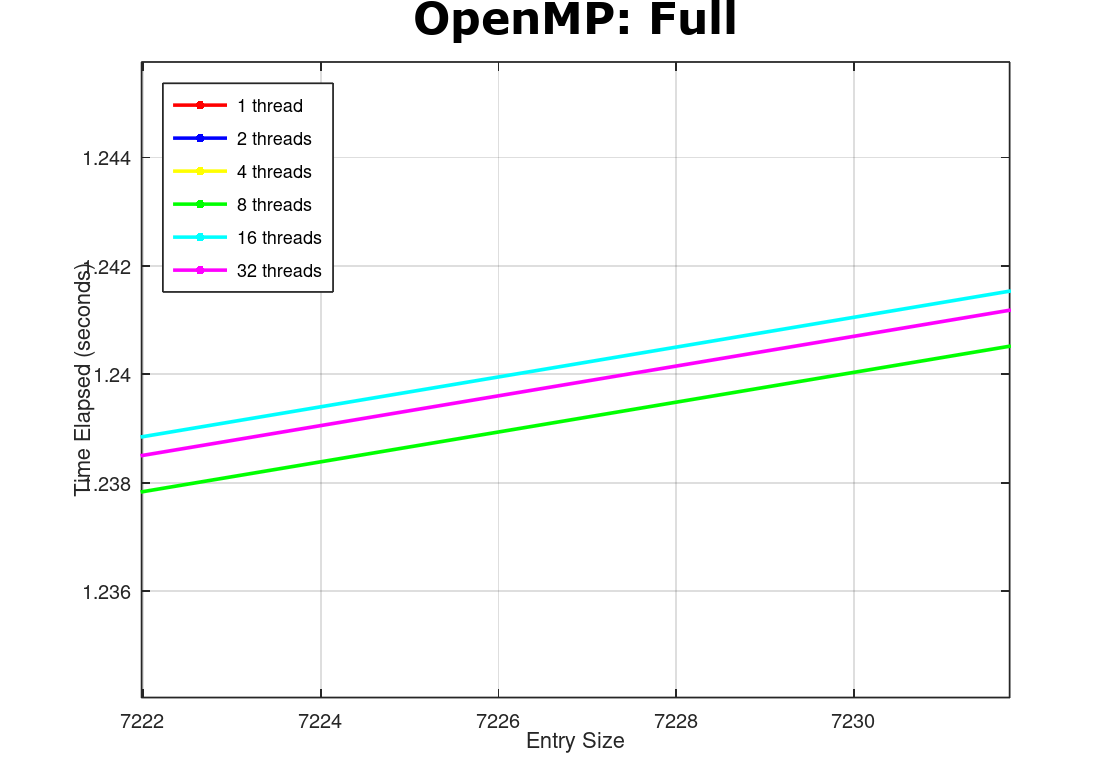
\includegraphics[scale=0.45]{omp_example}
	\caption{Grande zoom no gráfico referente ao caso OpenMP na região \textit{Full}.}
\end{figure}

De certa forma, isto indica que as diretivas de compilação do OpenMP tratam instruções de 8, 16 e 32 threads da mesma forma. Muito provavelmente isto aconteceu, pois o ambiente computacional em que realizamos os experimentos possuía uma CPU com 8 núcleos lógicos e, portanto, até 8 threads poderiam ser executadas simultaneamente (pelo menos em teoria).\\

Isto é compreensível, pois, sendo diretivas de compilação, o OpenMP pode extrair informações a nível de hardware (pelo compilador) para determinar o melhor executável a se gerar para a máquina em questão. Essa é a vantagem em relação ao Pthreads que foi mencionada: um melhor aproveitamento do hardware.\\

No entanto, isto gera uma dependência da performance ao sistema muito maior do que a normal. Neste sentido, Pthread se mostra mais portável que OpenMP. Uma anedota que exemplifica isto aconteceu durante a realização deste EP. Em outra máquina, quando estávamos implementando o caso OpenMP, tivemos dificuldade para executar com sucesso este caso e, quando conseguimos, o ganho em performance não foi tão expressivo.

\subsection{Analisando o caso Pthread}

Aqui, podemos somente pontuar que a melhor performance do caso OpenMP, em comparação ao caso Pthread, pode ser em decorrência de uma má implementação deste segundo método por nós. De todo modo, é inegável o grande ganho de performance em comparação a um caso sequencial.


\end{document}